\documentclass[aspectratio=169]{beamer}

\usepackage{amsmath}
\usepackage{tikz}
\usetikzlibrary{arrows.meta,calc,positioning}

\definecolor{inputblue}{RGB}{218,235,252}
\definecolor{gruorange}{RGB}{253,225,186}
\definecolor{headpurple}{RGB}{232,220,247}
\definecolor{gridgreen}{RGB}{214,239,221}
\definecolor{samplepink}{RGB}{249,218,225}

\setbeamercolor{frametitle}{fg=black}
\setbeamercolor{block title}{fg=black}

\tikzset{
  flow/.style={
    -{Latex[length=2.2mm]},
    line width=0.8pt,
    draw=black!75
  },
  recurrent/.style={
    -{Latex[length=2.2mm]},
    line width=0.8pt,
    draw=orange!75!black
  },
  modelnode/.style={
    draw=black!65,
    rounded corners=2pt,
    minimum height=1.15cm,
    align=center,
    font=\small
  },
  annotation/.style={
    align=center,
    font=\scriptsize,
    text=black!75
  }
}

\begin{document}

\begin{frame}{Bounded autoregressive trajectory model}
\centering

\resizebox{\textwidth}{!}{%
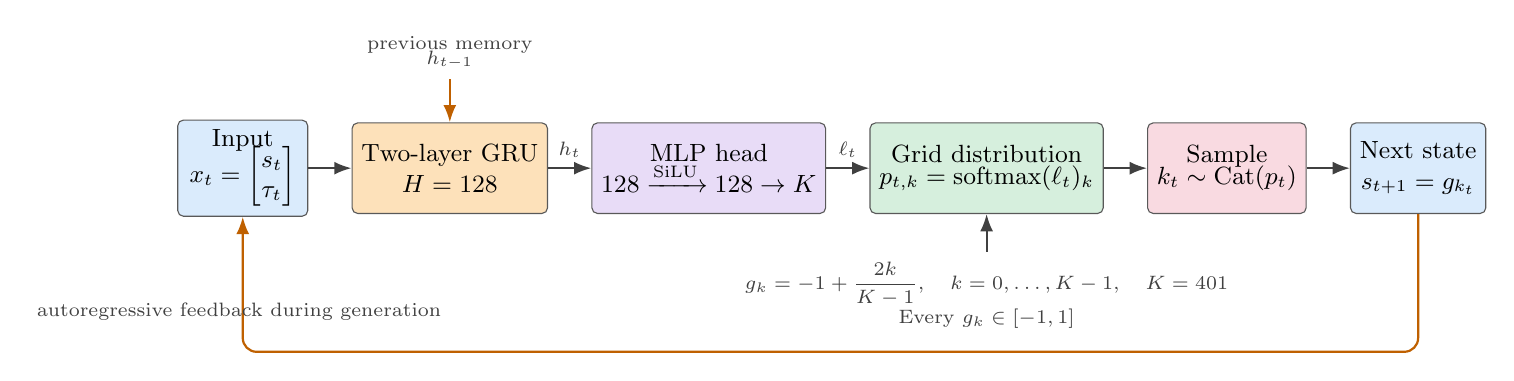
\begin{tikzpicture}[node distance=0.55cm]
  \node[
    modelnode,
    fill=inputblue,
    minimum width=1.65cm
  ] (input) {
    Input\\[-1mm]
    $\displaystyle x_t=
      \begin{bmatrix}s_t\\ \tau_t\end{bmatrix}$
  };

  \node[
    modelnode,
    fill=gruorange,
    minimum width=2.05cm,
    right=of input
  ] (gru) {
    Two-layer GRU\\
    $H=128$
  };

  \node[
    modelnode,
    fill=headpurple,
    minimum width=2.15cm,
    right=of gru
  ] (head) {
    MLP head\\
    $128\xrightarrow{\mathrm{SiLU}}128
      \rightarrow K$
  };

  \node[
    modelnode,
    fill=gridgreen,
    minimum width=1.85cm,
    right=of head
  ] (distribution) {
    Grid distribution\\[-1mm]
    $p_{t,k}=\operatorname{softmax}(\ell_t)_k$
  };

  \node[
    modelnode,
    fill=samplepink,
    minimum width=1.55cm,
    right=of distribution
  ] (sample) {
    Sample\\[-1mm]
    $k_t\sim\mathrm{Cat}(p_t)$
  };

  \node[
    modelnode,
    fill=inputblue,
    minimum width=1.35cm,
    right=of sample
  ] (nextstate) {
    Next state\\
    $s_{t+1}=g_{k_t}$
  };

  \draw[flow] (input) -- (gru);
  \draw[flow] (gru) -- node[above,annotation] {$h_t$} (head);
  \draw[flow] (head) -- node[above,annotation] {$\ell_t$} (distribution);
  \draw[flow] (distribution) -- (sample);
  \draw[flow] (sample) -- (nextstate);

  \node[annotation,above=0.55cm of gru] (previoushidden) {
    previous memory\\[-1mm]
    $h_{t-1}$
  };
  \draw[recurrent] (previoushidden.south) -- (gru.north);

  \node[annotation,below=0.48cm of distribution] (grid) {
    $\displaystyle
      g_k=-1+\frac{2k}{K-1},\quad
      k=0,\ldots,K-1,\quad K=401
    $\\
    Every $g_k\in[-1,1]$
  };
  \draw[flow] (grid.north) -- (distribution.south);

  \draw[recurrent,rounded corners=5pt]
    (nextstate.south)
    -- ++(0,-1.75)
    -| node[pos=0.72,below,annotation] {
      autoregressive feedback during generation
    }
    (input.south);
\end{tikzpicture}
}

\vspace{0.35cm}

\begin{block}{Training at every time step}
\small
\[
  y_t=s_{t+1}^{\mathrm{real}},
  \qquad
  q_{t,i}=1-\alpha,\quad q_{t,i+1}=\alpha,
  \qquad
  \mathcal{L}_t
  =-\sum_{k=0}^{K-1}q_{t,k}\log p_{t,k}.
\]
\vspace{-2mm}
\[
  \underbrace{\text{real }s_t\text{ as input}}_{\text{teacher forcing}}
  \quad\longrightarrow\quad
  \underbrace{\text{two-bin interpolated target }q_t}_{\text{continuous data on a discrete grid}}
  \quad\longrightarrow\quad
  \underbrace{\text{categorical cross-entropy}}_{\text{maximize next-state likelihood}} .
\]
\end{block}
\end{frame}

\end{document}
